\documentclass[tcc,capa]{texufpel}

\usepackage[utf8]{inputenc} % acentuacao
\usepackage{graphicx} % para inserir figuras
\usepackage[T1]{fontenc}
\usepackage{booktabs} % Para tabelas estéticas
\usepackage{float}    % Para posicionamento de figuras/tabelas
\usepackage{url}      % Para links nas referências

\hypersetup{
    hidelinks, % Remove coloração e caixas
    unicode=true,   %Permite acentuação no bookmark
    linktoc=all %Habilita link no nome e página do sumário
}

% -------------------------------------------------------------------------
% DADOS DO TRABALHO
% -------------------------------------------------------------------------
\unidade{Centro de Desenvolvimento Tecnológico}
\curso{Engenharia de Computação}
\nomecurso{Bacharelado em Engenharia de Computação}
\titulocurso{Bacharel em Engenharia de Computação}

\unidadeeng{Technology Development Center}
\cursoeng{Computer Engineering}

\title{Plataforma Híbrida de Instrumentação para Biosinais: Redução de Ruído com Hardware de Precisão e Inteligência Artificial}

\author{Menezes}{Gerson Leite de}
\advisor[Prof.~Dr.]{Rossetto}{Alan Carlos Junior}

% Palavras-chave em PT_BR
\keyword{instrumentação biomédica;}
\keyword{processamento de sinais;}
\keyword{inteligência artificial;}
\keyword{hardware de precisão.}

% Palavras-chave em EN_US
\keywordeng{biomedical instrumentation;}
\keywordeng{signal processing;}
\keywordeng{artificial intelligence;}
\keywordeng{precision hardware.}

\begin{document}

% Gera a capa e folha de rosto conforme o estilo texufpel
\maketitle 

\sloppy

% Ficha catalográfica (ajustar conforme biblioteca)
\fichacatalografica

% Folha de aprovação
\begin{aprovacao}{30 de Julho de 2026} 
\noindent Prof. Dr. Alan Carlos Junior Rossetto (orientador)\\
Doutor em Ciência da Computação pela UFRGS.\\[1cm]

\noindent Prof. Dr. Membro da Banca 1\\
Doutor em ... pela ...\\[1cm]

\noindent Prof. Dr. Membro da Banca 2\\
Doutor em ... pela ...\\[1cm]
\end{aprovacao}

% Dedicatória
\begin{dedicatoria}
  Dedico este trabalho aos meus pais e à minha namorada Gessyca, pelo apoio constante e incentivo durante toda a minha jornada acadêmica.
\end{dedicatoria}

% Agradecimentos
\begin{agradecimentos}
  Agradeço aos meus familiares e amigos, que sempre estiveram ao meu lado.
  Ao meu orientador, Prof. Alan Rossetto, pela oportunidade e confiança.
\end{agradecimentos}

% Epígrafe
\begin{epigrafe}
  ``A simplicidade é o grau máximo de sofisticação.''\\
  {\sc --- Leonardo da Vinci}
\end{epigrafe}

% -------------------------------------------------------------------------
% RESUMO
% -------------------------------------------------------------------------
\begin{abstract}
A aquisição de biosinais, como o Eletrocardiograma (ECG) e a Eletromiografia (EMG), é fundamental na saúde e pesquisa, mas estes sinais de baixa amplitude são suscetíveis a ruídos da rede elétrica e artefatos de movimento. Equipamentos profissionais de alta fidelidade possuem custo elevado, enquanto soluções de baixo custo carecem de precisão. Este trabalho propõe o desenvolvimento de uma plataforma híbrida de instrumentação para a aquisição e análise de biosinais, combinando um hardware de alta precisão com pós-processamento via software inteligente. A abordagem se baseia em duas frentes de atuação: primeiramente, o projeto de um \textit{shield} de condicionamento analógico de baixo ruído, responsável por amplificar e filtrar o sinal na sua origem. Em seguida, os dados adquiridos são processados em um computador por um algoritmo de Inteligência Artificial, que atua como uma segunda camada de filtragem adaptativa para atenuar ruídos complexos. Como principal contribuição, espera-se obter uma plataforma funcional de baixo custo que demonstre uma melhora significativa na relação sinal-ruído, validada através da aquisição de sinais reais de ECG e EMG.
\end{abstract}

% -------------------------------------------------------------------------
% ABSTRACT (INGLÊS)
% -------------------------------------------------------------------------
\begin{englishabstract}{Hybrid Instrumentation Platform for Biosignals: Noise Reduction with Precision Hardware and Artificial Intelligence}
The acquisition of biosignals, such as Electrocardiogram (ECG) and Electromyography (EMG), is fundamental in health and research, but these low-amplitude signals are susceptible to power line noise and motion artifacts. High-fidelity professional equipment is expensive, while low-cost solutions lack precision. This work proposes the development of a hybrid instrumentation platform for the acquisition and analysis of biosignals, combining high-precision hardware with intelligent software post-processing. The approach is based on two fronts: firstly, the design of a low-noise analog conditioning shield, responsible for amplifying and filtering the signal at its source. Next, the acquired data is processed on a computer by an Artificial Intelligence algorithm, acting as a second layer of adaptive filtering to attenuate complex noises. As a main contribution, a functional low-cost platform demonstrating a significant improvement in the signal-to-noise ratio is expected, validated through the acquisition of real ECG and EMG signals.
\end{englishabstract}

% Listas de Figuras e Tabelas
\listoffigures
\listoftables

% Lista de Abreviaturas
\begin{listofabbrv}{CMRR} % O parâmetro {CMRR} é a maior sigla para alinhar
    \item[ADC] Analog-to-Digital Converter
    \item[CMRR] Common-Mode Rejection Ratio
    \item[CNN] Convolutional Neural Network
    \item[DAE] Denoising Autoencoder
    \item[DAQ] Data Acquisition
    \item[ECG] Eletrocardiograma
    \item[EMG] Eletromiografia
    \item[ML] Machine Learning
    \item[IA] Inteligência Artificial
    \item[PCB] Printed Circuit Board
    \item[RNAs] Redes Neurais Artificiais
    \item[sEMG] Surface Electromyography
    \item[SNR] Signal-to-Noise Ratio
    \item[SoC] System on Chip
\end{listofabbrv}

% Sumário
\tableofcontents

% -------------------------------------------------------------------------
% CAPÍTULO 1: INTRODUÇÃO
% -------------------------------------------------------------------------
\chapter{Introdução}

A instrumentação biomédica dedica-se ao desenvolvimento de sistemas para medir e monitorar sinais fisiológicos. Dentre estes, os biopotenciais --- sinais elétricos gerados por atividade celular, como o Eletrocardiograma (ECG) e a Eletromiografia (EMG) --- são dos mais estudados e clinicamente relevantes. Historicamente, a aquisição destes sinais era restrita a ambientes clínicos controlados, utilizando equipamentos analógicos volumosos e de alto custo \cite{goldberger2000}.

Com o avanço da microeletrônica, tornou-se viável o desenvolvimento de sistemas de aquisição de dados (DAQ) portáteis e de baixo custo, frequentemente baseados em microcontroladores. Plataformas como o Arduino popularizaram o acesso a essas tecnologias. No entanto, a aquisição de biosinais apresenta um desafio de engenharia significativo: os sinais de interesse possuem amplitude muito baixa (na faixa de microvolts a milivolts) e seu espectro de frequência se sobrepõe a diversas fontes de ruído, notadamente o ruído da rede elétrica (60 Hz e seus harmônicos) e artefatos de movimento \cite{pathak2025}.

Soluções convencionais de baixo custo frequentemente falham em mitigar esse ruído de forma eficaz. O conversor Analógico-Digital (ADC) nativo de microcontroladores como o ATmega328 (do Arduino Uno) possui resolução e linearidade insuficientes, e o projeto de circuitos de condicionamento analógico --- a etapa de amplificação e filtragem que antecede a digitalização --- é crítico. Um projeto inadequado de \textit{front-end} analógico pode contaminar irremediavelmente o sinal antes mesmo que ele seja processado digitalmente \cite{kim2016}.

Por outro lado, o processamento digital de sinais e, mais recentemente, a Inteligência Artificial, trouxeram novas ferramentas para o tratamento de sinais ruidosos. Contudo, para ruídos complexos e não-estacionários, métodos de filtragem adaptativa \cite{widrow1975} e algoritmos baseados em aprendizado de máquina demonstram superioridade. Redes neurais, como as convolucionais (CNNs) e autoencoders, têm mostrado resultados promissores na reconstrução e remoção de ruído de sinais de ECG \cite{chandra2018, lomoio2024}.

Este trabalho se justifica pela lacuna existente entre os sistemas de instrumentação de baixo custo e a necessidade de alta fidelidade na aquisição de biosinais. A inovação do projeto reside na abordagem híbrida: em vez de depender unicamente do hardware ou do software, propõe-se uma sinergia entre ambos. O projeto se distingue de outros por não tentar corrigir um sinal de baixa qualidade (adquirido por hardware genérico) apenas com software. A hipótese é que, ao projetar um hardware de precisão dedicado (um \textit{shield} analógico de baixo ruído), o sinal entregue ao processador será de qualidade muito superior, permitindo que a camada de Inteligência Artificial atue de forma mais fina e eficaz.

\section{Objetivos}

\subsection{Objetivo Geral}
Desenvolver e validar uma plataforma híbrida de instrumentação para aquisição de biosinais (ECG e EMG), que utilize a sinergia entre um \textit{shield} de condicionamento analógico de precisão e algoritmos de Inteligência Artificial para maximizar a relação sinal-ruído.

\subsection{Objetivos Específicos}
\begin{itemize}
    \item Realizar um estudo aprofundado sobre a natureza dos biosinais, técnicas de condicionamento analógico e métodos de IA;
    \item Projetar e simular um circuito de \textit{front-end} analógico de baixo ruído, contendo amplificação de instrumentação e filtragem ativa;
    \item Implementar e validar o protótipo de hardware do \textit{shield}, primeiro em protoboard e, subsequentemente, em placa de circuito impresso (PCB);
    \item Desenvolver o software base de aquisição (firmware) e uma interface de visualização em tempo real;
    \item Implementar e treinar um modelo de Inteligência Artificial para a filtragem adaptativa de ruído;
    \item Integrar o hardware e o software em uma plataforma funcional;
    \item Validar o sistema completo através da aquisição de sinais reais, comparando quantitativamente a relação sinal-ruído.
\end{itemize}

% -------------------------------------------------------------------------
% CAPÍTULO 2: FUNDAMENTAÇÃO TEÓRICA
% -------------------------------------------------------------------------
\chapter{Fundamentação Teórica}

\section{Biosinais}
Os biosinais são registros de fenômenos biológicos que variam no tempo, podendo ser de natureza elétrica, mecânica ou química. No contexto deste trabalho, o foco recai sobre os biopotenciais, sinais elétricos gerados pela atividade eletroquímica de células excitáveis, especificamente o coração e os músculos esqueléticose eles serão obtidos através de eletrodos do tipo sEMG (Surface Electromyography)

\subsection{Eletrocardiograma (ECG)}
O Eletrocardiograma (ECG) é o registro gráfico da atividade elétrica do coração, captado por eletrodos posicionados na superfície corporal. Ele representa a soma espacial e temporal dos potenciais de ação das fibras miocárdicas durante o ciclo cardíaco. A análise morfológica do ECG é fundamental para o diagnóstico de diversas patologias, como arritmias, isquemias e infartos.

Segundo \cite{souto2016}, um ciclo cardíaco normal em um traçado de ECG é composto por uma sequência de deflexões características, denominadas ondas P, Q, R, S e T. A Onda P representa a despolarização atrial, ou seja, a ativação elétrica dos átrios que antecede a sua contração mecânica. É tipicamente uma onda arredondada e de pequena amplitude (0,1 a 0,2 mV). O Complexo QRS corresponde à despolarização ventricular. É a estrutura mais proeminente do ECG, caracterizada por uma deflexão rápida e de grande amplitude (até 1-2 mV), refletindo a grande massa muscular dos ventrículos. A Onda T representa a repolarização ventricular, momento em que o miocárdio recupera seu potencial de repouso para o próximo batimento.

\begin{figure}[htbp]
    \centering
    \includegraphics[width=0.8\textwidth]{imagens/ecg_padrao.png}
    \caption{Sinal de ECG típico mostrando as ondas P, QRS e T.}
    \label{fig:ecg}
\end{figure}

A padronização do registro de ECG é essencial para a análise clínica. O sinal é tradicionalmente impresso sobre uma grade milimetrada padrão, onde cada eixo possui um significado físico preciso. O eixo horizontal representa o tempo: a velocidade padrão de registro é de 25 mm/s. Assim, cada subdivisão menor (1 mm) corresponde a 0,04 segundos (40 ms), e cada quadrado maior (5 mm, composto por 5 quadradinhos) corresponde a 0,20 segundos (200 ms). O eixo vertical representa a voltagem (amplitude): a calibração padrão é de 10 mm/mV. Portanto, cada subdivisão menor (1 mm) na vertical representa 0,1 milivolts (0,1 mV), e cada quadrado maior (5 mm) representa 0,5 mV. Essa padronização permite que médicos e sistemas automatizados calculem a frequência cardíaca e a duração de intervalos críticos (como o intervalo PR e o segmento ST) visualmente.

\subsection{Eletromiografia (EMG)}
A eletromiografia (EMG) é uma técnica utilizada para o monitoramento da atividade elétrica das membranas excitáveis das células musculares. O sinal eletromiográfico representa a soma algébrica dos potenciais de ação das fibras musculares ativas detectados em uma determinada área \cite{marchetti2006}. Essa técnica é amplamente utilizada tanto em análises clínicas, como no estudo da marcha, quanto em aplicações de controle biomédico, pois fornece informações sobre o tempo de ativação e a intensidade da contração muscular.

Para a aquisição do sinal, comumente utilizam-se eletrodos de superfície (sEMG), que são dispositivos não invasivos aderidos à pele. A interface eletrodo-pele atua como um transdutor que capta a corrente iônica gerada nos músculos e a converte em corrente eletrônica para o sistema de instrumentação. Segundo \cite{marchetti2006}, a configuração bipolar é a mais adequada para esse tipo de aplicação. Nela, dois eletrodos de detecção são posicionados sobre o ventre muscular e um terceiro eletrodo (referência) é colocado em uma região eletricamente neutra. Essa configuração permite o uso de amplificação diferencial, fundamental para eliminar ruídos de modo comum que afetam ambos os eletrodos de detecção.

\begin{figure}[htbp]
    \centering
    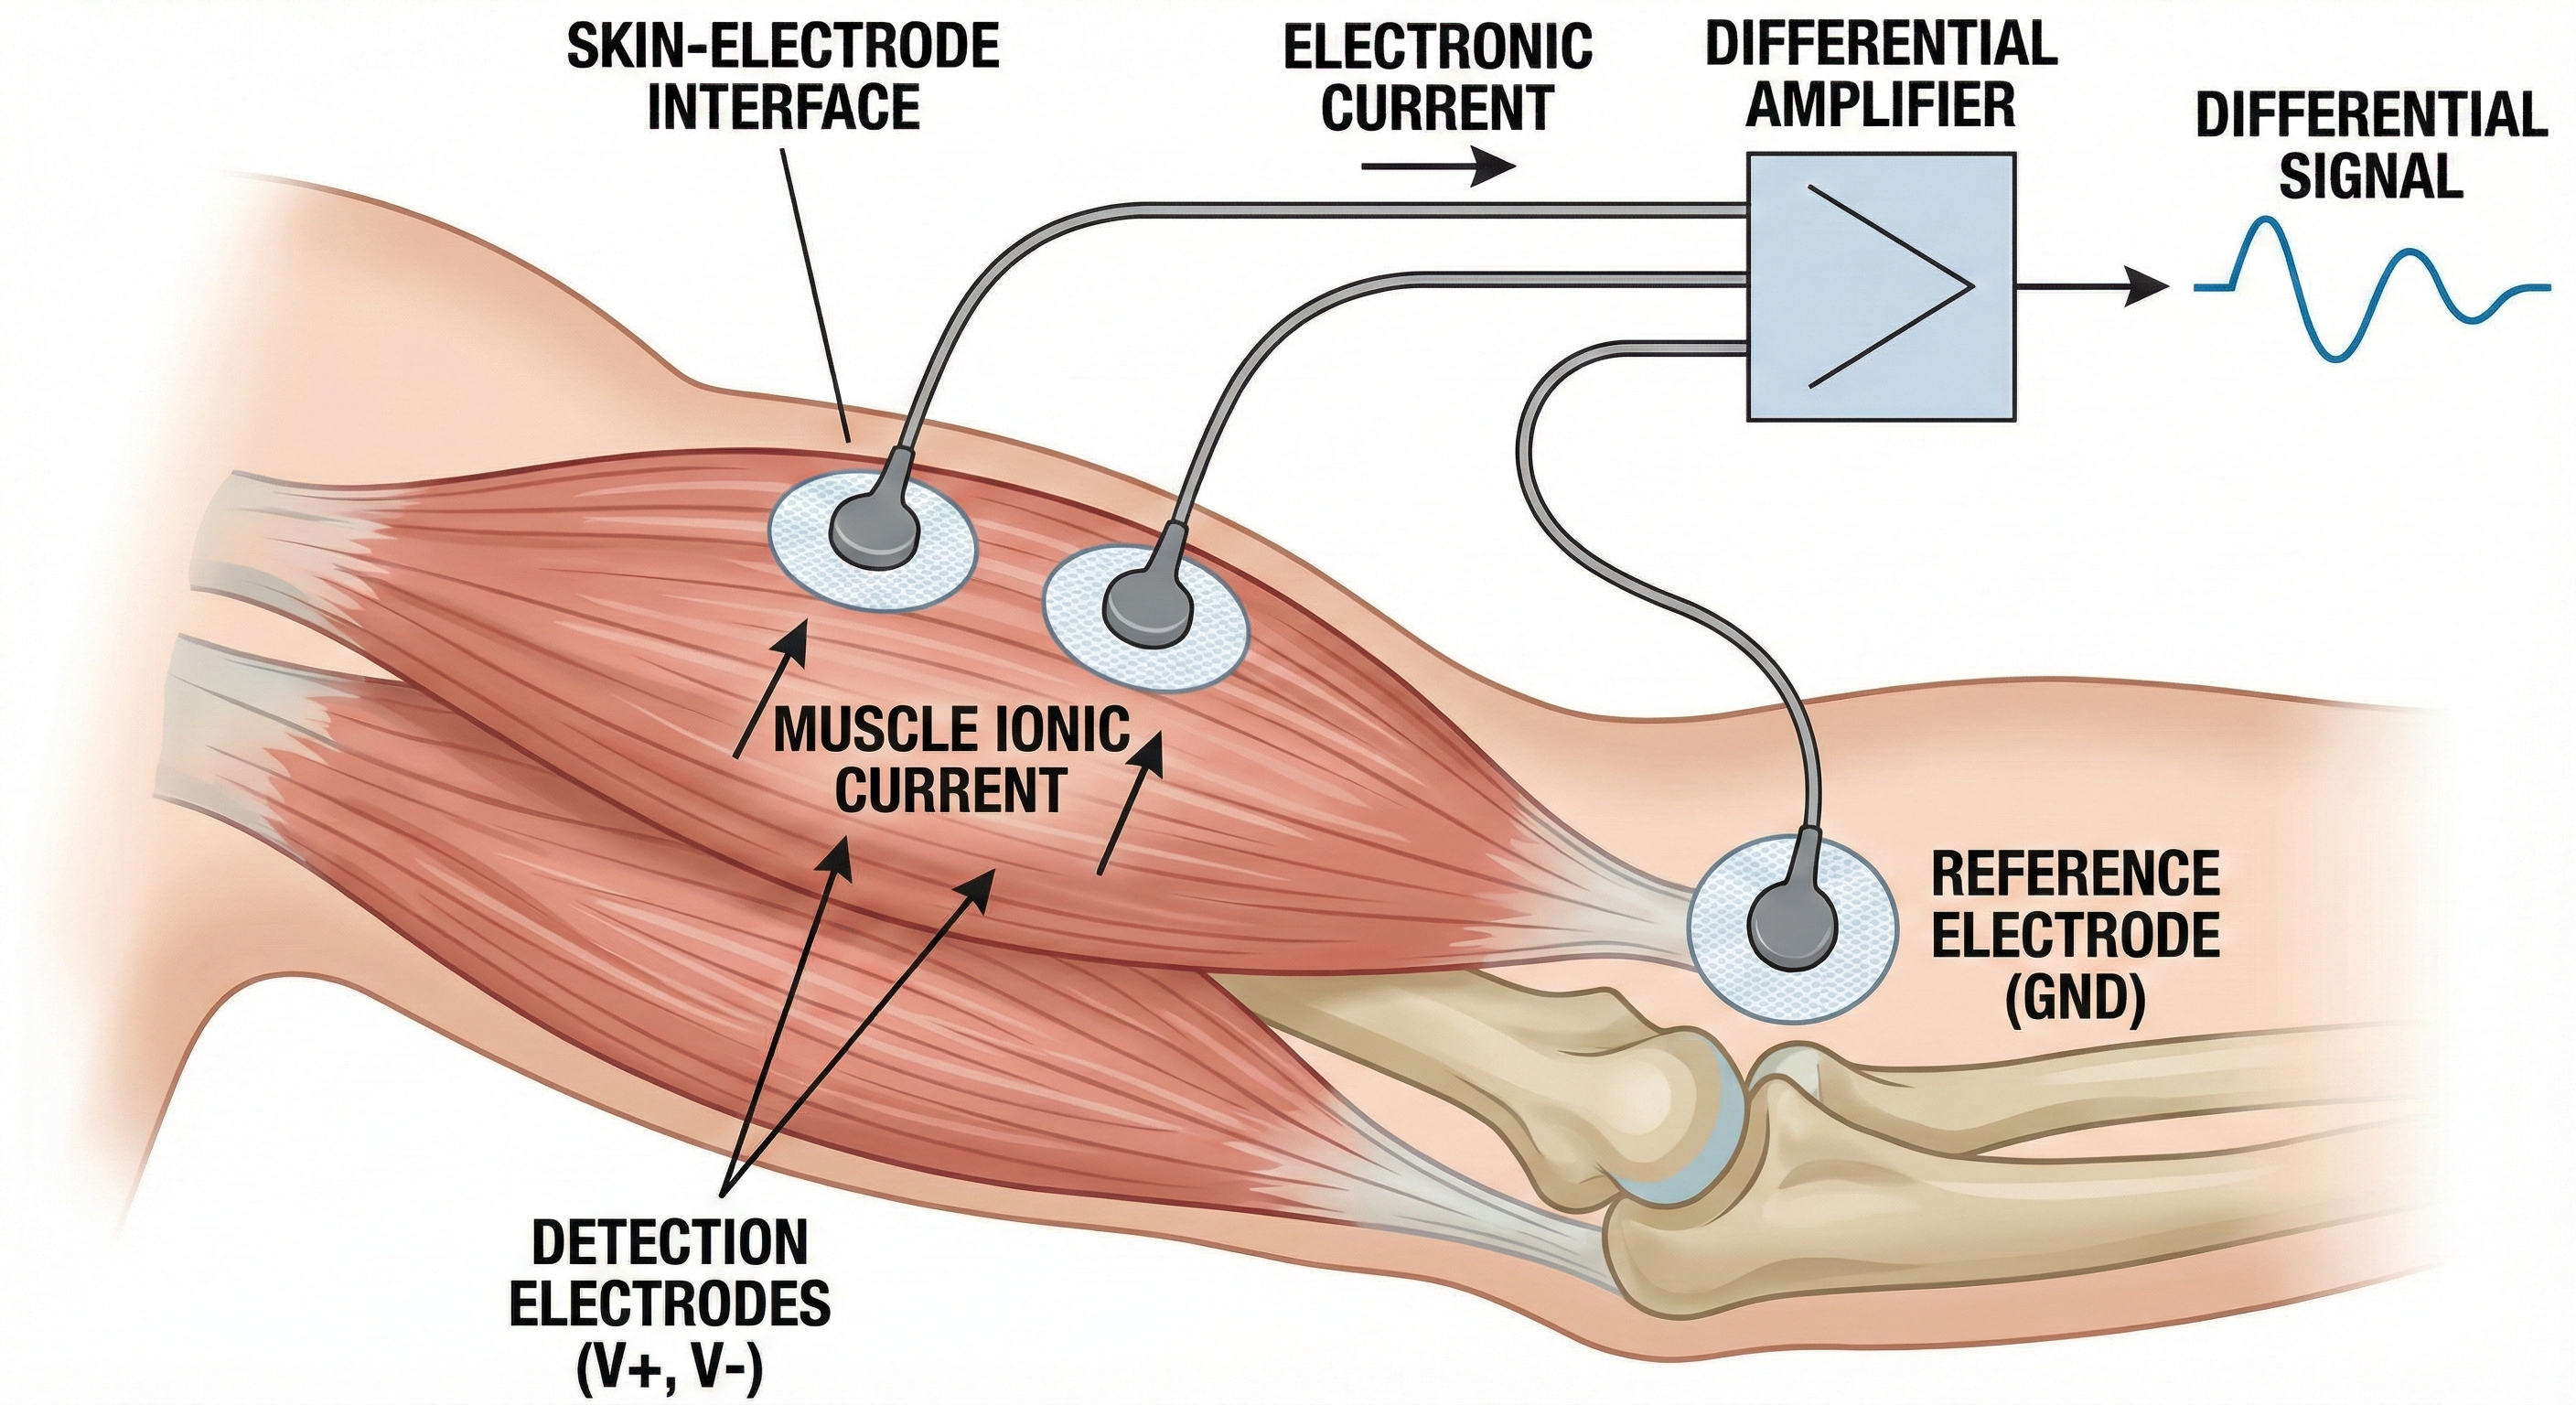
\includegraphics[width=0.8\textwidth]{imagens/eletrodo_illustration.png}
    \caption{Aquisição de biosinais utilizando-se eletrodos de superfícies}
    \label{fig:semg}
\end{figure}

O sinal de EMG bruto é estocástico e apresenta frequências que variam tipicamente entre 10 Hz e 500 Hz, com amplitudes na faixa de microvolts a milivolts \cite{marchetti2006}. Devido a essa natureza complexa, a análise do sinal geralmente requer processamento no domínio do tempo ou da frequência. Uma das técnicas mais comuns para quantificar a intensidade da ativação muscular é o cálculo do valor RMS (Root Mean Square), que reflete a potência do sinal sem a necessidade de retificação prévia, sendo uma métrica robusta para avaliar o nível de atividade elétrica muscular.

\section{Instrumentação e Condicionamento de Sinais}
Os sinais biológicos, como o ECG e o EMG, possuem amplitudes extremamente baixas e são frequentemente contaminados por ruídos externos e internos. Portanto, o estágio de instrumentação e condicionamento é crítico para garantir a integridade da informação antes que ela seja processada digitalmente. Esse processo envolve etapas principais de amplificação, filtragem e conversão analógico-digital.

A primeira etapa é a amplificação. Como os biopotenciais estão na ordem de milivolts ou microvolts, é necessário um ganho elevado para adequar o sinal à faixa dinâmica do conversor A/D. Para isso, utilizam-se amplificadores de instrumentação, que oferecem alta impedância de entrada — essencial para não carregar o circuito equivalente da pele — e uma alta Taxa de Rejeição de Modo Comum (CMRR). Um CMRR elevado (geralmente acima de 90 dB) é crucial para atenuar interferências eletromagnéticas, como o ruído de 60 Hz da rede elétrica, que incidem igualmente sobre os cabos e o corpo do paciente \cite{carr2001}.

Em seguida, o sinal passa pela filtragem. Filtros analógicos são empregados para limitar a largura de banda do sinal apenas às frequências de interesse biológico e para remover artefatos. No caso da eletromiografia, por exemplo, recomenda-se filtros passa-faixa para eliminar componentes de corrente contínua (DC) e ruídos de alta frequência. O filtro do tipo Butterworth é frequentemente citado na literatura, como em \cite{marchetti2006} e \cite{balbinot2019v1}), por apresentar uma resposta de frequência plana na banda de passagem, preservando a linearidade da amplitude do sinal biológico sem introduzir ripples (oscilações) indesejados.

Por fim, ocorre a Conversão Analógico-Digital (A/D). Esta etapa transforma o sinal contínuo de tensão em uma sequência discreta de números binários que podem ser processados por um microcontrolador ou computador. Dois parâmetros são fundamentais aqui: a resolução (número de bits), que define a menor variação de tensão detectável, e a frequência de amostragem. De acordo com o Teorema de Nyquist, a frequência de amostragem deve ser, no mínimo, o dobro da maior frequência contida no sinal para evitar o aliasing, um erro de reconstrução onde altas frequências são erroneamente interpretadas como baixas frequências \cite{marchetti2006}; \cite{balbinot2019v1}.

\section{Filtragem Digital e Inteligência Artificial}
\label{sec:filtragem_ia}

O tratamento de sinais biomédicos exige técnicas robustas para garantir que a informação fisiológica não seja mascarada por ruídos. Esta seção aborda desde os métodos clássicos de processamento digital até as abordagens modernas baseadas em aprendizado de máquina.

\subsection{Filtragem Digital}

A filtragem digital é o processo matemático realizado sobre um sinal discreto (amostrado) com o objetivo de modificar seu espectro de frequência, atenuando componentes indesejados e preservando a informação relevante. Segundo \cite{balbinot2019v1}, os filtros digitais são classificados fundamentalmente em duas categorias baseadas em sua resposta ao impulso: Filtros de Resposta ao Impulso Finita (FIR) e Filtros de Resposta ao Impulso Infinita (IIR). Os filtros FIR são inerentemente estáveis e possuem fase linear, o que é crucial para evitar distorções na morfologia de sinais como o ECG, embora exijam maior ordem (e custo computacional) para atingir cortes abruptos de frequência.

Já os filtros IIR, conforme explica \cite{balbinot2019v1}, conseguem mimetizar o comportamento de filtros analógicos clássicos (como Butterworth ou Chebyshev) com menor custo computacional e menor atraso de sinal. No entanto, eles podem apresentar instabilidade devido à realimentação e não possuem fase linear perfeita. Embora eficazes para ruídos estacionários (como a interferência de 60 Hz da rede elétrica), técnicas de filtragem digital clássica muitas vezes falham em remover artefatos não-estacionários e complexos, como o ruído de movimento muscular, sem degradar o sinal de interesse, o que motiva a busca por métodos adaptativos baseados em inteligência artificial.

\subsection{Inteligência Artificial (IA)}

A Inteligência Artificial (IA) pode ser definida como a capacidade de uma máquina realizar tarefas que, tradicionalmente, exigiriam inteligência humana. Isso inclui habilidades cognitivas como reconhecimento de padrões, compreensão de linguagem natural, percepção visual e tomada de decisão. O campo da IA é vasto e abrange subáreas como robótica, visão computacional e processamento de linguagem natural, buscando mimetizar a capacidade humana de raciocinar e interagir com o ambiente.

No contexto de biosinais, a IA permite que sistemas computacionais analisem grandes volumes de dados fisiológicos para identificar anomalias ou limpar sinais de forma mais eficiente que algoritmos determinísticos. Uma das vertentes mais promissoras para essa tarefa é o \textit{Deep Learning}, que utiliza estruturas matemáticas inspiradas no cérebro biológico para aprender representações complexas de dados a partir de exemplos, sem a necessidade de regras manuais rígidas.

\subsection{Aprendizado de Máquina (\textit{Machine Learning})}

O Aprendizado de Máquina, ou \textit{Machine Learning} (ML), é a ciência de fazer com que computadores ajam sem serem explicitamente programados para cada situação específica. É um subcampo da IA onde algoritmos analisam dados, aprendem com eles e fazem previsões ou decisões baseadas nos padrões encontrados. Segundo \cite{goodfellow2016}, as dificuldades enfrentadas por sistemas que dependem de conhecimento codificado rigidamente sugerem que os sistemas de IA precisam da capacidade de adquirir seu próprio conhecimento, extraindo padrões de dados brutos. Essa capacidade é conhecida como aprendizado de máquina.

Computadores são historicamente eficientes em tarefas que podem ser formalizadas matematicamente, mas falham em tarefas subjetivas ou intuitivas para humanos, como reconhecer um rosto ou interpretar um sinal ruidoso. O ML resolve isso através de paradigmas de aprendizado, que podem ser: supervisionado (onde o sistema é treinado com pares de entrada-saída rotulados), não supervisionado (onde o sistema busca estruturas ocultas em dados não rotulados) e aprendizado por reforço (baseado em recompensas e punições). Essa capacidade de generalização permite categorizar objetos, prever tendências futuras e, no escopo deste trabalho, distinguir entre o sinal cardíaco real e o ruído de fundo.

\subsection{Redes Neurais Artificiais}

As Redes Neurais Artificiais (RNAs) são modelos computacionais inspirados no funcionamento do sistema nervoso central humano. Elas são compostas por unidades de processamento elementares, chamadas de neurônios artificiais, que são interconectadas através de canais de comunicação associados a valores numéricos conhecidos como "pesos". O princípio básico é que a rede aprende ajustando esses pesos: cada vez que um caminho leva a uma decisão correta durante o treinamento, as conexões envolvidas são fortalecidas matematicamente.

Uma RNA é tipicamente organizada em camadas: uma camada de entrada (que recebe os dados brutos), uma ou mais camadas ocultas (onde ocorre o processamento e extração de características) e uma camada de saída. Cada neurônio processa seus dados de entrada através de uma função de ativação não-linear e transmite o resultado para a próxima camada. Essa arquitetura permite que a rede modele relações complexas e não-lineares entre as entradas e as saídas, sendo ideal para o processamento de sinais biológicos que variam dinamicamente.

\subsection{Aprendizado Profundo (\textit{Deep Learning})}

O \textit{Deep Learning} (Aprendizado Profundo) é uma subárea do \textit{Machine Learning} que se concentra no treinamento de redes neurais com muitas camadas ocultas (daí o termo "profundo"). Segundo \cite{dsa2022}, essa profundidade permite que o algoritmo modele e aprenda representações dos dados em múltiplos níveis de abstração. Enquanto as camadas iniciais podem aprender a detectar pequenas variações locais no sinal, as camadas mais profundas combinam essas informações para reconhecer morfologias complexas, como o complexo QRS de um ECG.

Para viabilizar o \textit{Deep Learning}, é necessário um grande volume de dados para treinamento e um alto poder computacional, frequentemente suprido pelo uso de Unidades de Processamento Gráfico (GPUs), que aceleram as operações matriciais massivas envolvidas no processo. Conforme \cite{goodfellow2016}, o \textit{Deep Learning} resolve o problema central da aprendizagem de representações, permitindo que o computador construa conceitos complexos a partir de conceitos mais simples, superando a performance de algoritmos tradicionais em tarefas de percepção como visão e audição.

\subsection{Redes Neurais Convolucionais (CNNs)}

As Redes Neurais Convolucionais (CNNs) são uma classe especializada de redes neurais profundas, projetadas originalmente para processar dados que possuem uma topologia de grade, como imagens bidimensionais (2D). No entanto, elas têm se mostrado extremamente eficazes para o processamento de séries temporais unidimensionais (1D), como os sinais de ECG e EMG \cite{lomoio2024}. A principal característica das CNNs é o uso da operação matemática de convolução, onde filtros (ou \textit{kernels}) deslizam sobre o sinal de entrada para extrair características locais relevantes, independentemente de sua posição no tempo, conferindo invariância à translação.

Em aplicações de \textit{denoising} (remoção de ruído) de biosinais, as CNNs 1D conseguem aprender a morfologia das ondas características, como a onda R do ECG, e diferenciá-las de ruídos aleatórios \cite{lomoio2024}. A arquitetura típica envolve camadas de convolução para extração de \textit{features}, seguidas por camadas de \textit{pooling} (subamostragem), que reduzem a dimensionalidade e aumentam a robustez do modelo a pequenas variações temporais, permitindo uma filtragem adaptativa que preserva a forma do sinal clínico \cite{goodfellow2016, lomoio2024}.

\subsection{Autoencoders}

Os Autoencoders são um tipo de rede neural utilizada para aprendizado não supervisionado, cujo objetivo principal é aprender uma representação compacta (codificação) dos dados de entrada. A arquitetura de um autoencoder é composta por duas partes principais: o \textit{Encoder}, que comprime a entrada em uma representação de menor dimensão (espaço latente), e o \textit{Decoder}, que tenta reconstruir a entrada original a partir dessa representação comprimida. O aprendizado ocorre minimizando a diferença entre a entrada e a saída reconstruída.

Para a redução de ruído, utiliza-se uma variação conhecida como \textit{Denoising Autoencoder} (DAE). Neste método, o modelo é treinado introduzindo-se propositalmente ruído no sinal de entrada, mas forçando a rede a compará-lo com o sinal limpo na saída. Com isso, o Autoencoder é obrigado a aprender as características estruturais robustas do biosinal (como a periodicidade do ECG) e a ignorar o ruído, pois o ruído é aleatório e não possui padrão passível de compressão eficiente no espaço latente. Isso torna os DAEs ferramentas poderosas para limpar sinais biomédicos degradados \cite{lomoio2024}.
% -------------------------------------------------------------------------
% CAPÍTULO 3: TRABALHOS RELACIONADOS
% -------------------------------------------------------------------------
\chapter{Trabalhos Relacionados}

Diversos trabalhos na literatura abordam a aquisição e filtragem de biosinais, explorando tanto melhorias em hardware quanto em software. \cite{kim2016} propuseram um SoC (\textit{System on Chip}) reconfigurável para aquisição de biosinais em plataformas vestíveis de baixa potência, focando na eficiência energética do hardware analógico integrado.

No contexto de melhoria de hardware discreto, \cite{goel2013} e, mais recentemente, \cite{pathak2025} discutiram o design de amplificadores operacionais de baixo ruído especificamente para instrumentação biomédica, demonstrando a importância da escolha de componentes e topologias de baixo ruído (\textit{low-noise}) para garantir a fidelidade do sinal antes da digitalização.

Em relação ao processamento via software, \cite{singh2019} exploraram uma técnica baseada em transformada wavelet modificada para remoção de ruído em ECG, obtendo bons resultados em ruídos gaussianos. Avançando para o uso de \textit{Deep Learning}, \cite{chandra2018} utilizaram Redes Neurais Recorrentes (RNNs) para limpeza de sinal. Mais recentemente, \cite{lomoio2024} desenvolveram o DCAE-SR, um Autoencoder Convolucional para reconstrução de sinais de ECG em super-resolução, evidenciando o potencial de redes neurais profundas na recuperação de detalhes finos do sinal que seriam perdidos por filtros convencionais.

O presente trabalho difere destes por propor uma arquitetura que integra ambas as pontas: um \textit{front-end} analógico customizado de alta precisão (não integrado em SoC fechado) aliado a modelos de IA modernos, visando uma plataforma aberta, de baixo custo e replicável.

% -------------------------------------------------------------------------
% CAPÍTULO 4: DESENVOLVIMENTO
% -------------------------------------------------------------------------
\chapter{Metodologia e Desenvolvimento}

Esta seção documenta o desenvolvimento da primeira etapa prevista no cronograma: a definição da arquitetura do sistema. São apresentados a definição da topologia adotada, o detalhamento dos blocos funcionais e a seleção dos componentes eletrônicos críticos.

\section{Definição de Topologia}

Para o desenvolvimento de sistemas de instrumentação biomédica, a literatura apresenta diferentes abordagens de topologia. Após análise comparativa de viabilidade e desempenho, optou-se pela **Topologia Híbrida (Condicionamento Analógico + Processamento Remoto)**.

Nesta arquitetura, o \textit{hardware} analógico (o \textit{shield} proposto) realiza o condicionamento crítico (amplificação de instrumentação e filtragem de frequências espúrias), entregando um sinal limpo e com amplitude adequada ao conversor A/D. O processamento digital pesado (IA) é delegado a um computador, permitindo o uso de algoritmos complexos sem restrições de \textit{hardware} embarcado.

Esta decisão permite usar microcontroladores de baixo custo (como interface) e aproveitar o poder computacional do PC para a Inteligência Artificial, garantindo que o sinal chegue ao conversor A/D já com boa qualidade.

\section{Detalhamento dos Blocos do Sistema}

A arquitetura do sistema foi dividida em quatro macro-blocos funcionais, conforme descrito a seguir:

\begin{enumerate}
    \item \textbf{Bloco de Aquisição Analógica (\textit{Front-End}):} Responsável pela interface com o paciente. Utiliza um Amplificador de Instrumentação (INA) para garantir alta Razão de Rejeição em Modo Comum (CMRR), eliminando interferências de rede elétrica. Inclui estágios de filtragem ativa (Passa-Alta e Passa-Baixa) para delimitar a banda de frequência dos biosinais.
    
    \item \textbf{Bloco de Conversão e Controle:} Composto pelo microcontrolador e um Conversor Analógico-Digital (ADC) externo. Este bloco digitaliza o sinal condicionado e o transmite via protocolo serial. O uso de um ADC externo visa superar as limitações de resolução (10 bits) e ruído dos conversores internos de microcontroladores comuns.
    
    \item \textbf{Bloco de Comunicação:} Interface (USB/Serial) que transporta o fluxo de dados digitais do \textit{hardware} para a estação de trabalho.
    
    \item \textbf{Bloco de Processamento Inteligente (Software):} Executado em computador, responsável por receber os dados, realizar o pré-processamento digital e aplicar o modelo de Inteligência Artificial (Autoencoder) para a remoção final de artefatos complexos e visualização.
\end{enumerate}

\section{Definição dos Componentes Eletrônicos Críticos}

A escolha dos componentes foi baseada na necessidade de baixo ruído e alta fidelidade, conforme os objetivos do projeto. A Tabela \ref{tab:componentes} resume os componentes selecionados.

\begin{table}[H]
\centering
\caption{Definição dos Componentes Críticos do Hardware}
\label{tab:componentes}
\begin{tabular}{p{4cm} p{3cm} p{7cm}}
\toprule
\textbf{Função} & \textbf{Componente} & \textbf{Justificativa Técnica} \\
\midrule
Amplificação de Instrumentação & AD620 & Padrão em instrumentação médica devido ao alto CMRR ($>100$ dB) e ganho ajustável com um único resistor externo. \\
\midrule
Filtragem Ativa (Op-Amps) & OPA2134 & O OPA2134 oferece baixíssima distorção e ruído, ideal para áudio e biosinais. O TL074 é uma alternativa de baixo custo com entrada JFET e alta impedância. \\
\midrule
Conversão A/D (ADC) & ADS1115 & Módulo ADC de 16-bits com interface I2C. Proporciona uma resolução significativamente superior aos 10-bits nativos do Arduino, essencial para capturar micro-variações do sinal. \\
\midrule
Microcontrolador & Arduino Uno R3 & Atua como plataforma de controle e interface I2C para o ADC, facilitando a integração e prototipagem rápida proposta na metodologia. \\
\midrule
Isolação de Energia & B0505S-1W & Conversor DC-DC isolado para separar a alimentação do circuito analógico da USB, reduzindo ruído digital. \\
\bottomrule
\end{tabular}
\end{table}

% RESULTADOS
\chapter{Resultados}

% CONCLUSÃO
\chapter{Conclusão}

% Bibliografia
\bibliographystyle{abnt}
\bibliography{bibliografia} 

\end{document}